\documentclass{standalone}
\usepackage{tikz}
\usetikzlibrary{patterns, positioning}


\begin{document}
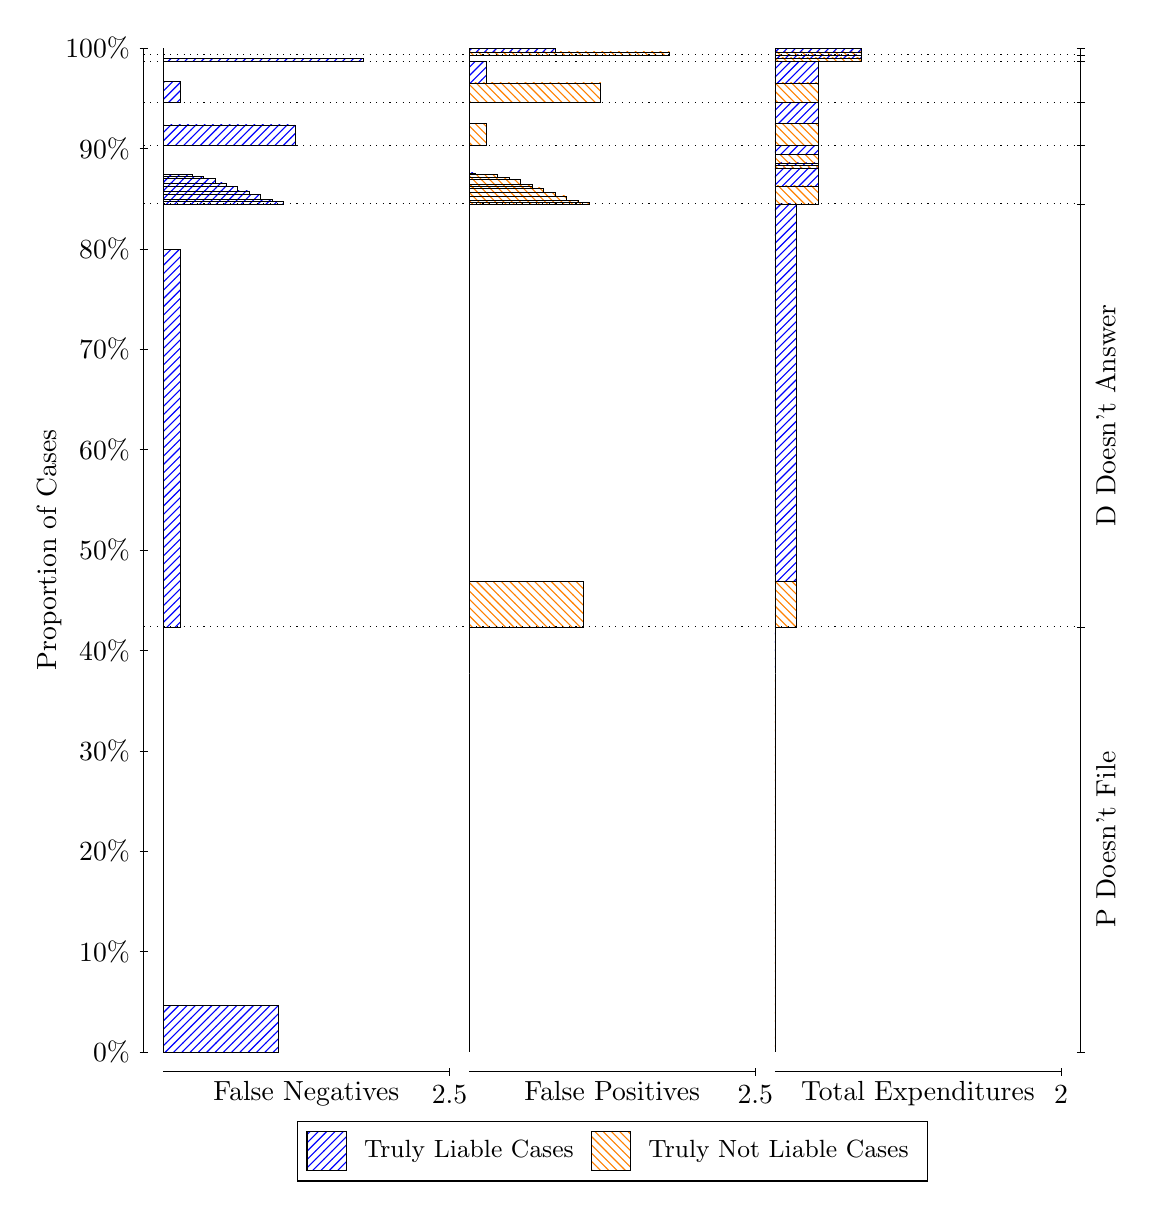
\begin{tikzpicture}
\draw[black, very thin] (1.5,1.75) -- (1.5,14.5);
\node[rotate=90, text=black, anchor=center] at (0.3, 8.125) {Proportion of Cases};
\draw[black, very thin] (1.45,1.75) -- (1.55,1.75);
\node[text=black, anchor=east] at (1.45, 1.75) {0\%};
\draw[black, very thin] (1.45,3.025) -- (1.55,3.025);
\node[text=black, anchor=east] at (1.45, 3.025) {10\%};
\draw[black, very thin] (1.45,4.3) -- (1.55,4.3);
\node[text=black, anchor=east] at (1.45, 4.3) {20\%};
\draw[black, very thin] (1.45,5.575) -- (1.55,5.575);
\node[text=black, anchor=east] at (1.45, 5.575) {30\%};
\draw[black, very thin] (1.45,6.85) -- (1.55,6.85);
\node[text=black, anchor=east] at (1.45, 6.85) {40\%};
\draw[black, very thin] (1.45,8.125) -- (1.55,8.125);
\node[text=black, anchor=east] at (1.45, 8.125) {50\%};
\draw[black, very thin] (1.45,9.4) -- (1.55,9.4);
\node[text=black, anchor=east] at (1.45, 9.4) {60\%};
\draw[black, very thin] (1.45,10.675) -- (1.55,10.675);
\node[text=black, anchor=east] at (1.45, 10.675) {70\%};
\draw[black, very thin] (1.45,11.95) -- (1.55,11.95);
\node[text=black, anchor=east] at (1.45, 11.95) {80\%};
\draw[black, very thin] (1.45,13.225) -- (1.55,13.225);
\node[text=black, anchor=east] at (1.45, 13.225) {90\%};
\draw[black, very thin] (1.45,14.5) -- (1.55,14.5);
\node[text=black, anchor=east] at (1.45, 14.5) {100\%};

\draw[black, very thin] (13.4,1.75) -- (13.4,14.5);
\draw[black, very thin] (13.35,1.75) -- (13.45,1.75);
\node[anchor=west] at (13.35, 1.75) {};
\draw[black, very thin] (13.35,7.1479) -- (13.45,7.1479);
\node[anchor=west] at (13.35, 7.1479) {};
\draw[black, very thin] (13.35,12.52) -- (13.45,12.52);
\node[anchor=west] at (13.35, 12.52) {};
\draw[black, very thin] (13.35,13.266) -- (13.45,13.266);
\node[anchor=west] at (13.35, 13.266) {};
\draw[black, very thin] (13.35,13.806) -- (13.45,13.806);
\node[anchor=west] at (13.35, 13.806) {};
\draw[black, very thin] (13.35,14.328) -- (13.45,14.328);
\node[anchor=west] at (13.35, 14.328) {};
\draw[black, very thin] (13.35,14.414) -- (13.45,14.414);
\node[anchor=west] at (13.35, 14.414) {};
\draw[black, very thin] (13.35,14.5) -- (13.45,14.5);
\node[anchor=west] at (13.35, 14.5) {};

\draw[black, very thin, pattern color=blue, pattern=north east lines] (1.75,1.75) rectangle (3.2033,2.3394);
\draw[black, very thin, pattern color=orange, pattern=north west lines] (1.75,2.3394) rectangle (1.75,7.1479);
\draw[black, very thin, pattern color=blue, pattern=north east lines] (1.75,7.1479) rectangle (1.968,11.943);
\draw[black, very thin, pattern color=orange, pattern=north west lines] (1.75,11.943) rectangle (1.75,12.52);
\draw[black, very thin, pattern color=blue, pattern=north east lines] (1.75,12.52) rectangle (3.276,12.549);
\draw[black, very thin, pattern color=blue, pattern=north east lines] (1.75,12.549) rectangle (3.1307,12.579);
\draw[black, very thin, pattern color=blue, pattern=north east lines] (1.75,12.579) rectangle (2.9853,12.646);
\draw[black, very thin, pattern color=blue, pattern=north east lines] (1.75,12.646) rectangle (2.84,12.686);
\draw[black, very thin, pattern color=blue, pattern=north east lines] (1.75,12.686) rectangle (2.6947,12.746);
\draw[black, very thin, pattern color=blue, pattern=north east lines] (1.75,12.746) rectangle (2.5493,12.787);
\draw[black, very thin, pattern color=blue, pattern=north east lines] (1.75,12.787) rectangle (2.404,12.849);
\draw[black, very thin, pattern color=blue, pattern=north east lines] (1.75,12.849) rectangle (2.2587,12.872);
\draw[black, very thin, pattern color=blue, pattern=north east lines] (1.75,12.872) rectangle (2.1133,12.893);
\draw[black, very thin, pattern color=orange, pattern=north west lines] (1.75,12.893) rectangle (1.75,13.266);
\draw[black, very thin, pattern color=blue, pattern=north east lines] (1.75,13.266) rectangle (3.4213,13.525);
\draw[black, very thin, pattern color=orange, pattern=north west lines] (1.75,13.525) rectangle (1.75,13.806);
\draw[black, very thin, pattern color=blue, pattern=north east lines] (1.75,13.806) rectangle (1.968,14.078);
\draw[black, very thin, pattern color=orange, pattern=north west lines] (1.75,14.078) rectangle (1.75,14.328);
\draw[black, very thin, pattern color=blue, pattern=north east lines] (1.75,14.328) rectangle (4.2933,14.367);
\draw[black, very thin, pattern color=orange, pattern=north west lines] (1.75,14.367) rectangle (1.75,14.414);
\draw[black, very thin, pattern color=orange, pattern=north west lines] (1.75,14.414) rectangle (1.75,14.452);
\draw[black, very thin, pattern color=blue, pattern=north east lines] (1.75,14.452) rectangle (1.75,14.5);
\draw[black, very thin, pattern color=orange, pattern=north west lines] (5.6333,1.75) rectangle (5.6333,6.5585);
\draw[black, very thin, pattern color=blue, pattern=north east lines] (5.6333,6.5585) rectangle (5.6333,7.1479);
\draw[black, very thin, pattern color=orange, pattern=north west lines] (5.6333,7.1479) rectangle (7.0867,7.7245);
\draw[black, very thin, pattern color=blue, pattern=north east lines] (5.6333,7.7245) rectangle (5.6333,12.52);
\draw[black, very thin, pattern color=orange, pattern=north west lines] (5.6333,12.52) rectangle (7.1593,12.538);
\draw[black, very thin, pattern color=orange, pattern=north west lines] (5.6333,12.538) rectangle (7.014,12.561);
\draw[black, very thin, pattern color=orange, pattern=north west lines] (5.6333,12.561) rectangle (6.8687,12.623);
\draw[black, very thin, pattern color=orange, pattern=north west lines] (5.6333,12.623) rectangle (6.7233,12.664);
\draw[black, very thin, pattern color=orange, pattern=north west lines] (5.6333,12.664) rectangle (6.578,12.724);
\draw[black, very thin, pattern color=orange, pattern=north west lines] (5.6333,12.724) rectangle (6.4327,12.748);
\draw[black, very thin, pattern color=orange, pattern=north west lines] (5.6333,12.748) rectangle (6.4327,12.764);
\draw[black, very thin, pattern color=orange, pattern=north west lines] (5.6333,12.764) rectangle (6.2873,12.831);
\draw[black, very thin, pattern color=orange, pattern=north west lines] (5.6333,12.831) rectangle (6.142,12.861);
\draw[black, very thin, pattern color=orange, pattern=north west lines] (5.6333,12.861) rectangle (5.9967,12.894);
\draw[black, very thin, pattern color=blue, pattern=north east lines] (5.6333,12.894) rectangle (5.706,12.915);
\draw[black, very thin, pattern color=blue, pattern=north east lines] (5.6333,12.915) rectangle (5.6333,13.266);
\draw[black, very thin, pattern color=orange, pattern=north west lines] (5.6333,13.266) rectangle (5.8513,13.547);
\draw[black, very thin, pattern color=blue, pattern=north east lines] (5.6333,13.547) rectangle (5.6333,13.806);
\draw[black, very thin, pattern color=orange, pattern=north west lines] (5.6333,13.806) rectangle (7.3047,14.056);
\draw[black, very thin, pattern color=blue, pattern=north east lines] (5.6333,14.056) rectangle (5.8513,14.328);
\draw[black, very thin, pattern color=orange, pattern=north west lines] (5.6333,14.328) rectangle (5.6333,14.375);
\draw[black, very thin, pattern color=blue, pattern=north east lines] (5.6333,14.375) rectangle (5.6333,14.414);
\draw[black, very thin, pattern color=orange, pattern=north west lines] (5.6333,14.414) rectangle (8.1767,14.452);
\draw[black, very thin, pattern color=blue, pattern=north east lines] (5.6333,14.452) rectangle (6.7233,14.5);
\draw[black, very thin, pattern color=orange, pattern=north west lines] (9.5167,1.75) rectangle (9.5167,6.5585);
\draw[black, very thin, pattern color=blue, pattern=north east lines] (9.5167,6.5585) rectangle (9.5167,7.1479);
\draw[black, very thin, pattern color=orange, pattern=north west lines] (9.5167,7.1479) rectangle (9.7892,7.7245);
\draw[black, very thin, pattern color=blue, pattern=north east lines] (9.5167,7.7245) rectangle (9.7892,12.52);
\draw[black, very thin, pattern color=orange, pattern=north west lines] (9.5167,12.52) rectangle (10.062,12.748);
\draw[black, very thin, pattern color=blue, pattern=north east lines] (9.5167,12.748) rectangle (10.062,12.978);
\draw[black, very thin, pattern color=orange, pattern=north west lines] (9.5167,12.978) rectangle (10.062,13.011);
\draw[black, very thin, pattern color=blue, pattern=north east lines] (9.5167,13.011) rectangle (10.062,13.04);
\draw[black, very thin, pattern color=orange, pattern=north west lines] (9.5167,13.04) rectangle (10.062,13.153);
\draw[black, very thin, pattern color=blue, pattern=north east lines] (9.5167,13.153) rectangle (10.062,13.266);
\draw[black, very thin, pattern color=orange, pattern=north west lines] (9.5167,13.266) rectangle (10.062,13.547);
\draw[black, very thin, pattern color=blue, pattern=north east lines] (9.5167,13.547) rectangle (10.062,13.806);
\draw[black, very thin, pattern color=orange, pattern=north west lines] (9.5167,13.806) rectangle (10.062,14.056);
\draw[black, very thin, pattern color=blue, pattern=north east lines] (9.5167,14.056) rectangle (10.062,14.328);
\draw[black, very thin, pattern color=orange, pattern=north west lines] (9.5167,14.328) rectangle (10.607,14.375);
\draw[black, very thin, pattern color=blue, pattern=north east lines] (9.5167,14.375) rectangle (10.607,14.414);
\draw[black, very thin, pattern color=orange, pattern=north west lines] (9.5167,14.414) rectangle (10.607,14.452);
\draw[black, very thin, pattern color=blue, pattern=north east lines] (9.5167,14.452) rectangle (10.607,14.5);
\draw[black, dotted] (1.5,7.1479) -- (13.4,7.1479);
\draw[black, dotted] (1.5,12.52) -- (13.4,12.52);
\draw[black, dotted] (1.5,13.266) -- (13.4,13.266);
\draw[black, dotted] (1.5,13.806) -- (13.4,13.806);
\draw[black, dotted] (1.5,14.328) -- (13.4,14.328);
\draw[black, dotted] (1.5,14.414) -- (13.4,14.414);
\draw[black, very thin] (1.75,1.5) -- (5.3833,1.5);
\node[text=black, anchor=north] at (3.5667, 1.5) {False Negatives};
\draw[black, very thin] (5.3833,1.45) -- (5.3833,1.55);
\node[text=black, anchor=north] at (5.3833, 1.45) {2.5};

\draw[black, very thin] (5.6333,1.5) -- (9.2667,1.5);
\node[text=black, anchor=north] at (7.45, 1.5) {False Positives};
\draw[black, very thin] (9.2667,1.45) -- (9.2667,1.55);
\node[text=black, anchor=north] at (9.2667, 1.45) {2.5};

\draw[black, very thin] (9.5167,1.5) -- (13.15,1.5);
\node[text=black, anchor=north] at (11.333, 1.5) {Total Expenditures};
\draw[black, very thin] (13.15,1.45) -- (13.15,1.55);
\node[text=black, anchor=north] at (13.15, 1.45) {2};

\node[text=black, centered, rotate=90] at (13.72, 4.449) {P Doesn't File};
\node[text=black, centered, rotate=90] at (13.72, 9.834) {D Doesn't Answer};






\draw (7.449999999999999,1.5) node[draw=none] (baseCoordinate) {};
\begin{scope}[align=center]
        \matrix[scale=0.5, draw=black, below=0.5cm of baseCoordinate, nodes={draw}, column sep=0.1cm]{
            \node[rectangle, draw, minimum width=0.5cm, minimum height=0.5cm, pattern color=blue, pattern=north east lines] {}; &
            \node[draw=none, font=\small, text=black] (B) {Truly Liable Cases}; &
            \node[rectangle, draw, minimum width=0.5cm, minimum height=0.5cm, pattern color=orange, pattern=north west lines] {}; &
            \node[draw=none, font=\small, text=black] (B) {Truly Not Liable Cases}; \\
            };
\end{scope}

\end{tikzpicture}
\end{document}